% TODO: 
% - Motivation - das kann man noch deutlich besser machen. (Aber wie?)
% - „Graphen-Zoo“ (K_n, C_n, P_n, ...)


\section{Graphen}

\begin{frame}{Ein Graph}
	
	\begin{figure}[H]
		\begin{tikzpicture}[->,>=stealth,baseline=-5mm]
		\matrix[matrix of math nodes,nodes={draw,circle,minimum size=10mm,inner sep=2pt},row sep=15mm,column sep=15mm,ampersand replacement=\&]
		{
			|(1)| 1 \& |(3)| 3 \\
			|(0)| 0 \& |(2)| 2  \\
		};
		\draw  (0) -- (1);
		\draw  (1) -- (2);
		\draw  (2) -- (3);
		\draw  (3) -- (1);
		
		\end{tikzpicture}
	\end{figure}
	
\end{frame}

\begin{frame}{Graphen -- Wofür?}
	\begin{itemize}
		\item Straßennetze und andere Verkehrsnetze (Kürzeste Wege)
		\item Kabelnetze (Minimale Spannbäume)
		\item Rohrnetze (Maximaler Fluss)
	\end{itemize}

	\begin{block}{Zitat}
		\enquote{Egal für wie wichtig du Graphen in der Informatik hältst, sie sind mindestens doppelt so wichtig!}\\
		\emph{Ein Google-Manager über Einstellungsgespräche bei Google}
	\end{block}
\end{frame}

\subsection{Definitionen}

\begin{frame}{Graphen}
	\begin{Definition}
		Ein \textbf{gerichteter Graph} ist ein Paar $G = (V, E)$ mit einer \emph{endlichen}, \emph{nichtleeren} Menge an \textbf{Knoten} $V$ und einer Menge an \textbf{Kanten}\\
		$E \subseteq V \times V$.
	\end{Definition} \pause
	$E$ enthält also Paare (geordnet) von Elementen aus $V$. \pause
	
	\bigskip
	\begin{Definition}
		Ein \textbf{ungerichteter Graph} ist ein Paar $G = (V, E)$ mit einer \emph{endlichen}, \emph{nichtleeren} Menge an \textbf{Knoten} $V$ und einer Menge an \textbf{Kanten}\\
		$E \subseteq \set{ \{x,y\} \Mid x \in V \land y \in V }$.
	\end{Definition} \pause
	$E$ enthält also Mengen (ungeordnet) mit je ein oder zwei Elementen aus $V$!
\end{frame}

\begin{frame}{Graphen}
	\begin{block}{Hinweis}
		Häufig wählt man $V = \Z_k = \{0,1,2,...,k-1\}$\\
		
		Da $V$ immer endlich ist, muss auch $E$ endlich sein.\\
		$E = \emptyset$ geht aber!
	\end{block}

	\pause
	\begin{Definition}
		Eine Kante mit identischem Start- und Endpunkt nennt man \textbf{Schlinge}.\\
		Also $(x,x) \in E$ (gerichtet) bzw. $\{x\} \in E$ (ungerichtet).\\
		\smallskip
		
		Zwei Knoten $x$ und $y$ in einem Graphen $G$ heißen \textbf{adjazent}, wenn eine Kante von $x$ nach $y$ zeigt.
	\end{Definition}
	% \textbf{Achtung}: Im gerichteten Fall ist diese Aussage nicht symmetrisch!
	% Das stimmt zwar, hat in den letzten zwei Jahren aber mehr verwirrt als geholfen, denn dann kommt gleich die Frage "und wie rum muss man das jetzt sagen...".

	\pause

	\begin{block}{Hinweis}
		Einen gerichteten Graphen $G = (V,E)$ kann man in den \textbf{zu $G$ gehörigen ungerichteten Graphen} umwandeln, indem man die Pfeilspitzen weglässt. \\
		Andersrum: Aus einer Kante zwei machen mit Pfeilen in beide Richtungen.
	\end{block}
\end{frame}

\begin{frame}{Beispiel}
	Wir betrachten den gerichteten Graphen $G = (V, E)$ mit $V = \{0,1,2,3,4,5\}$ und $E = \set{(0,1), (1,0), (1,2), (3,4), (4,3) ,(4,5)}$
	\bigskip

	\begin{figure}[H]
		\begin{tikzpicture}[->,>=stealth,baseline=-5mm]
		\matrix[matrix of math nodes,nodes={draw,circle,minimum size=10mm,inner sep=2pt},row sep=15mm,column sep=15mm,ampersand replacement=\&]
		{
			|(1)| 1 \& |(5)| 5 \& |(3)| 3 \\
			|(0)| 0 \& |(2)| 2 \& |(4)| 4 \\
		};
		\draw  (0) to [bend left] (1);
		\draw  (1) to [bend left] (0);
		\draw  (1) -- (2);
		
		\draw  (4) -- (5);
		\draw  (4) to [bend left] (3);
		\draw  (3) to [bend left] (4);
		\end{tikzpicture}
	\end{figure}

\end{frame}

\begin{frame}{Aufgabe: Graphen zeichnen}
	Zeichnet die Graphen $G_i = (V, E_i)$ mit $V = \Z_4$ und
	$E_1 = \set{(0,1), (0,2), (0,3), (1,2), (1,3), (2,2), (2,3), (3,2)}$\\
	$E_2 = \set{\{0,1\}, \{0,2\}, \{0,3\} }$\\
	$E_3 = \emptyset$\\
	$E_4 = V \times V$\\
	$E_5 = \set{(0,1), (1,2), (1,3)}$
\end{frame}

\begin{frame}[t]{Lösung: Graphen zeichnen}
	Zeichnet den Graphen $G_1 = (V, E_1)$ mit
	$$V = \Z_4 \qquad E_1 = \set{(0,1), (0,2), (0,3), (1,2), (1,3), (2,2), (2,3), (3,2)}$$
	
	\pause
	\bigskip
	\begin{figure}[H]
		\begin{tikzpicture}[->,>=stealth,baseline=-5mm]
			\matrix[matrix of math nodes,nodes={draw,circle,minimum size=10mm,inner sep=2pt},row sep=15mm,column sep=15mm,ampersand replacement=\&]
			{
				|(0)| 0 \& |(1)| 1 \& |(2)| 2 \\
				\& |(3)| 3 \& \\
			};
			\draw  (0) -- (1);
			\draw  (0) -- (3);
			\draw  (2)  to [bend left] (3);
			\draw  (1) -- (2);
			\draw  (3) to [bend left] (2);
			\draw  (0) to [bend left]  (2);
			\path (2) edge [loop right] ();
			\draw (1) -- (3);
		\end{tikzpicture}
	\end{figure}
\end{frame}

\begin{frame}[t]{Lösung: Graphen zeichnen}
	Zeichnet den Graphen $G_2 = (V, E_2)$ mit
	$$V = \Z_4 \qquad E_2 = \set{\{0,1\}, \{0,2\}, \{0,3\} }$$
	
	\pause
	\bigskip
	\begin{figure}[H]
		\begin{tikzpicture}[-,>=stealth,baseline=-5mm]
		\matrix[matrix of math nodes,nodes={draw,circle,minimum size=10mm,inner sep=2pt},row sep=15mm,column sep=15mm,ampersand replacement=\&]
		{
			|(0)| 0 \& |(1)| 1 \& |(2)| 2 \\
			\& |(3)| 3 \& \\
		};
		\draw  (0) -- (1);
		\draw  (0)  to [bend left] (2);
		\draw  (0) -- (3);
		\end{tikzpicture}
	\end{figure}
\end{frame}

\begin{frame}[t]{Lösung: Graphen zeichnen}
	Zeichnet den Graphen $G_3 = (V, E_3)$ mit
	$$V = \Z_4 \qquad E_3 = \emptyset$$
	
	\pause
	\bigskip
	\begin{figure}[H]
		\begin{tikzpicture}[->,>=stealth,baseline=-5mm]
		\matrix[matrix of math nodes,nodes={draw,circle,minimum size=10mm,inner sep=2pt},row sep=15mm,column sep=15mm,ampersand replacement=\&]
		{
			|(0)| 0 \& |(1)| 1 \& |(2)| 2 \\
			\& |(3)| 3 \& \\
		};
		\end{tikzpicture}
	\end{figure}
\end{frame}

\def\bend{8}
\begin{frame}[t]{Lösung: Graphen zeichnen}
	Zeichnet den Graphen $G_4 = (V, E_4)$ mit
	$$V = \Z_4 \qquad E_4 = V \times V$$
	
	\pause
	\bigskip  %TODO!!
	\begin{figure}[H]
		\begin{tikzpicture}[->,>=stealth,baseline=-5mm]
		\matrix[matrix of math nodes,nodes={draw,circle,minimum size=10mm,inner sep=2pt},row sep=25mm,column sep=25mm,ampersand replacement=\&]
		{
			|(0)| 0 \& |(1)| 1 \\
			|(2)| 2 \& |(3)| 3 \\
		};
		\path (0) edge [loop left] ();
		\path (1) edge [loop right] ();
		\path (2) edge [loop left] ();
		\path (3) edge [loop right] ();
		
		\draw  (0) to [bend left=\bend] (1);
		\draw  (0) to [bend left=\bend] (2);
		\draw  (0) to [bend left=\bend] (3);
		\draw  (1) to [bend left=\bend] (0);
		\draw  (1) to [bend left=\bend] (2);
		\draw  (1) to [bend left=\bend] (3);
		\draw  (2) to [bend left=\bend] (0);
		\draw  (2) to [bend left=\bend] (1);
		\draw  (2) to [bend left=\bend] (3);
		\draw  (3) to [bend left=\bend] (0);
		\draw  (3) to [bend left=\bend] (1);
		\draw  (3) to [bend left=\bend] (2);
		
		
		\end{tikzpicture}
	\end{figure}
\end{frame}

\begin{frame}[t]{Lösung: Graphen zeichnen}
	Zeichnet den Graphen $G_5 = (V, E_5)$ mit
	$$V = \Z_4 \qquad E_5 = \set{ (0,1), (1,2), (1,3) }$$
	
	\pause
	\bigskip
	\begin{figure}[H]
		\begin{tikzpicture}[->,>=stealth,baseline=-5mm]
		\matrix[matrix of math nodes,nodes={draw,circle,minimum size=10mm,inner sep=2pt},row sep=15mm,column sep=15mm,ampersand replacement=\&]
		{
			|(0)| 0 \& |(1)| 1 \& |(2)| 2 \\
			\& |(3)| 3 \& \\
		};
		\draw  (0) -- (1);
		\draw  (1) -- (2);
		\draw  (1) -- (3);
		\end{tikzpicture}
	\end{figure}
\end{frame}


\begin{frame}{Teilgraphen}
	\begin{Definition}
		Ein \textbf{Teilgraph} $T = (V',E')$ von $G$ ist ein Graph, den man kriegt, wenn man aus $G$ beliebige Knoten und Kanten so wegwirft, dass keine Kante \enquote{in die Luft} zeigt.  Also (für gerichtete Graphen):
		%Ein \textbf{Teilgraph} $T = (V',E')$ von $G$ ist ein Graph, bei dem Knoten- und Kantenmenge Teilmengen des Graphens $G$ sind und deren Kanten nicht aus dem Teilgraph hinausführen. Also (für gerichtete Graphen):
		$$V' \subseteq V \qquad E' \subseteq E \cap (V' \times V')$$
	\end{Definition} \pause

	Hinweis: Natürlich dürfen wir in $E'$ auch Kanten aus $E \cap (V' \times V')$ \enquote{weglassen}!
\end{frame}

\begin{frame}{Teilgraphen: Beispiel}
	\begin{columns}
		\column[T]{0.3 \linewidth}
		
		\begin{tikzpicture}[->,>=stealth,baseline=-5mm]
		\matrix[matrix of math nodes,nodes={draw,circle,minimum size=5mm,inner sep=2pt},row sep=10mm,column sep=10mm,ampersand replacement=\&]
		{
			|(0)| 0 \& |(1)| 1 \& |(2)| 2 \\
			\& |(3)| 3 \& \\
		};
		\draw  (0) -- (1);
		\draw  (0) -- (3);
		\draw  (2)  to [bend left] (3);
		\draw  (1) -- (2);
		\draw  (3) to [bend left] (2);
		\draw  (0) to [bend left]  (2);
		\path (2) edge [loop right] ();
		\draw (1) -- (3);
		\end{tikzpicture}
		\begin{center}
			Graph $G$
		\end{center}
		
		\pause
		\column[T]{0.3 \linewidth}
		\begin{tikzpicture}[->,>=stealth,baseline=-5mm]
		\matrix[matrix of math nodes,nodes={draw,circle,minimum size=5mm,inner sep=2pt},row sep=10mm,column sep=10mm,ampersand replacement=\&]
		{
			|(0)| 0 \& |(1)| 1 \& |(2)| 2 \\
			\&  \& \\
		};
		\draw  (0) -- (1);
		\draw  (1) -- (2);
		\draw  (0) to [bend left]  (2);
		\end{tikzpicture}
		\begin{center}
			Teilgraph $T_1$ von $G$
		\end{center}
		
		\pause
		\column[T]{0.3 \linewidth}
		\begin{tikzpicture}[->,>=stealth,baseline=-5mm]
		\matrix[matrix of math nodes,nodes={draw,circle,minimum size=5mm,inner sep=2pt},row sep=10mm,column sep=10mm,ampersand replacement=\&]
		{
			|(0)| 0 \& |(1)| 1 \& |(2)[white]| 2 \\  % (2): stealth node
			        \& |(3)| 3 \& \\
		};
		\draw[->, white]  (0) to [bend left] (2); % stealth edge
		\draw  (0) -- (1);
		\draw  (0) -- (3);
		\draw (1) -- (3);
		\end{tikzpicture} 
		\begin{center}
			Teilgraph $T_2$ von $G$
		\end{center}
	\end{columns}
\end{frame}

\begin{frame}{Teilgraphen: Beispiel}
	\begin{columns}
		\column[T]{0.3 \linewidth}
		
		\begin{tikzpicture}[->,>=stealth,baseline=-5mm]
		\matrix[matrix of math nodes,nodes={draw,circle,minimum size=5mm,inner sep=2pt},row sep=10mm,column sep=10mm,ampersand replacement=\&]
		{
			|(0)| 0 \& |(1)| 1 \& |(2)| 2 \\
			\& |(3)| 3 \& \\
		};
		\draw  (0) -- (1);
		\draw  (0) -- (3);
		\draw  (2)  to [bend left] (3);
		\draw  (1) -- (2);
		\draw  (3) to [bend left] (2);
		\draw  (0) to [bend left]  (2);
		\path (2) edge [loop right] ();
		\draw (1) -- (3);
		\end{tikzpicture}
		\begin{center}
			Graph $G$
		\end{center}
		
		\column[T]{0.5 \linewidth}
		\begin{tikzpicture}[->,>=stealth,baseline=-5mm]
		\matrix[matrix of math nodes,nodes={draw,circle,minimum size=5mm,inner sep=2pt},row sep=10mm,column sep=10mm,ampersand replacement=\&]
		{
			|(2)[white]| 2  \& |(0)| 0 \& |(1)[white]| 1 \\ % (1), (2): stealth nodes
			\& \& |(3)[white]| 3  \\
		};
		\draw[myalertcolor]  (0) -- (1);
		\draw[myalertcolor]  (0) -- (3);
		\draw[->, white]  (2) to [bend left] (1); % stealth edge
		\end{tikzpicture}
		\begin{center}
			...ist überhaupt kein Graph \\ \impl auch kein Teilgraph!
		\end{center}
	\end{columns}	
\end{frame}

\begin{frame}{Knotengrade}
	
	\begin{Definition}
		In \emph{gerichteten} Graphen:
		Der \textbf{Eingangsgrad} eines Knoten $k$ ist die Anzahl der Kanten, die auf $k$ zeigen. \\
		Der \textbf{Ausgangsgrad} eines Knoten $k$ ist die Anzahl der Kanten, die von $k$ wegzeigen.  Also: 
		\begin{align*}
			d^-(k) = \abs{\set{ x \Mid (x,k) \in E}} \\
			d^+(k) = \abs{\set{ x \Mid (k,x) \in E}}
		\end{align*}
		\pause
		Der \textbf{Grad} eines Knotens $k$ ist $d(k) = d^+(k) + d^-(k)$.
	\end{Definition}

	\pause
	\bigskip
	In \emph{ungerichteten} Graphen (bei uns!):\\
	Knotengrad $d(k)$ ist Anzahl der \enquote{Linien}, die $k$ berühren.\\
	Schlingen zählen also zweifach!
	%Also tatsächlich \enquote{Anzahl der Berührungen von Linien mit dem Kreis}.
\end{frame}

\begin{frame}{Aufgabe: Maximale Kanten}
	Sei $G$ ein \textbf{gerichteter} Graph mit $n$ Knoten. Wie viele Kanten kann $G$ maximal haben... \\[0.2in]
	
	Wenn Schlingen erlaubt sind? \pause \\ 
	$n^2$  \\[0.3in]
	
	Wenn er schlingenfrei ist? \pause\\ 
	$n^2 - n = n \* (n-1)$		
\end{frame}

\begin{frame}{Aufgabe: Maximale Kanten}
	Sei $G$ ein \textbf{ungerichteter} Graph mit $n$ Knoten. Wie viele Kanten kann $G$ maximal haben... \\[0.2in]
	
	\visible<3->{Wenn Schlingen erlaubt sind? \\ }
	\visible<4->{$\frac{n(n+1)}{2} \qquad \left( = \frac{n(n-1)}{2} + n\right)$ \\[0.3in]}
	
	Wenn er schlingenfrei ist? \\
	\visible<2->{$\frac{n(n-1)}{2} $\\ Man verbindet jeden Knoten mit den jeweils anderen Knoten, fasst dann jeweils 2 gleiche Kanten zusammen.}
\end{frame}

\subsection{Pfade und Wege}
\begin{frame}{Pfade und Wege}
	\begin{Definition}
		Sei $G$ ein \emph{gerichteter / ungerichteter} Graph.\\
		Ein \textbf{Pfad / Weg} ist eine Folge von Knoten, die jeweils über Kanten im Graphen erreichbar sind. Also eine \alert{nichtleere} Liste $$p = (v_0, v_1, \dots, v_n) \quad \text{mit} \quad (v_i, v_{i+1}) \in E$$
	\end{Definition}
	\pause
	Die Länge eines Pfades ist die Anzahl der Kanten \quad $n = \abs{p} - 1$ \; (!). \\
	\smallskip
	$w$ heißt \textbf{von $v$ erreichbar}, wenn es einen Pfad von $v$ nach $w$ gibt.
	\begin{Beispiel}
		Sei $G = (V, E)$ mit $V = \Z_9, \quad E = V \times V$\\ \pause
		$p_1 = (7)$ ist ein Pfad der Länge 0.\\
		$p_2 = (0, 1, 2, 3, 0)$ ist ein Pfad der Länge 4.
	\end{Beispiel}
\end{frame}

\begin{frame}[t]{Pfade}
	Sei $G$ ein gerichteter Graph.{\hphantom{un}} Ein Pfad $p = (v_0, \dots, v_n)$ heißt
	\begin{tabular}{>{\itshape}rp{.7\textwidth}}
		geschlossen & wenn $v_0 = v_n$ gilt  \\
		Zyklus & wenn er geschlossen ist und Länge $\geq 1$ gilt \\
		wiederholungsfrei & Wenn alle Knoten paarweise verschieden sind \newline ($v_0 = v_n$ geht aber!) \\
		einfacher Zyklus &  wenn er ein wiederholungsfreier Zyklus ist  \\
	\end{tabular}
	\medskip \\
	\textbf{Azyklischer} Graph: Graph ohne Zyklen\\
	\impl Oftmals auch DAG (Directed Acyclic Graph)
\end{frame}

\begin{frame}[t]{Wege}
	Sei $G$ ein \alert{un}gerichteter Graph. Ein \alert{Weg} $p = (v_0, \dots, v_n)$ heißt
	\begin{tabular}{>{\itshape}rp{.7\textwidth}}
		geschlossen & wenn $v_0 = v_n$ gilt  \\
		\alert{Kreis} & wenn er geschlossen ist und Länge $\geq 1$ gilt \\
		wiederholungsfrei & Wenn alle Knoten paarweise verschieden sind \newline ($v_0 = v_n$ geht aber!) \\
		einfacher \alert{Kreis} &  wenn er ein wiederholungsfreier Kreis \alert{mit mind. 3~versch. Knoten} ist  \\
	\end{tabular}

\end{frame}

\begin{frame}{Teilpfade}
	\begin{Definition}
		Ein \emph{Teilpfad} eines Pfades entsteht durch Streichen von Knoten am Anfang und/oder Ende des Pfades.
	\end{Definition}

	\pause
	\begin{block}{Beachte}
		Mindestens einen Knoten übrig lassen! (Sonst kein gültiger Pfad mehr)\\
		Es darf \textbf{nicht} aus der Mitte gestrichen werden! (Sonst evtl. kein Pfad mehr, wenn die entsprechenden Kanten nicht im Graphen vorhanden sind)
	\end{block}

	\pause
	\begin{Beispiel}
		Sei $p = (1, 2, 3, 4, 5, 1)$ und $G$ passend gewählt.\\
		\pause
		$(2, 3), (1, 2, 3, 4, 5), (4, 5, 1)$ sind Teilpfade\\
		$(), (1, 2, 1), (1, 2, 3, 4, 5, 1, 2)$ sind keine Teilpfade.
	\end{Beispiel}
\end{frame}

%TODO Beispiel Pfade
%Beispiel machen, in dem zwar ein Pfad von x nach y existiert, aber nicht umgekehrt.
%• beachte: für aufeinanderfolgende Knoten im Pfad muss die Kante in die richtige Richtung
%weisen!
%• Beachte: Knoten dürfen in Pfad mehrfach vorkommen
%• Beispiel machen, in dem von x nach y unterschiedlich lange Pfade vorkommen

\begin{frame}{Isomorphie}
	Zwei Graphen heißen \textbf{isomorph}, wenn sie \enquote{bis auf eine Umbenennung der Knoten identisch sind}, also die gleiche Struktur besitzen.\\
	
	\pause
	\medskip
	
	Formal: Haben $G_1 = (V_1, E_1), \, G_2 = (V_2, E_2)$. \\ \smallskip
	$G_1$ \textbf{isomorph} zu $G_2$, wenn es eine Bijektion $f \from V_1 \functionto V_2$ gibt mit \[\forall x,y \in V_1: \quad (x,y) \in E_1 \gdw \tuple{f(x),f(y)} \in E_2. \]
	
	$f$ heißt dann auch \emph{(Graph-)Isomorphismus}.
	
\end{frame}

\begin{frame}{Aufgabe: Graphisomorphie}
	\begin{block}{Aufgabe (WS 2010)}
		Jeweils zwei der sechs Graphen sind isomorph zueinander. Geben Sie die Paare von isomorphen Graphen sowie den zugehörigen Isomorphismus ($=$~„Umbenennung“) in Tabellenform an.
		\begin{figure}[H]
			\centering
			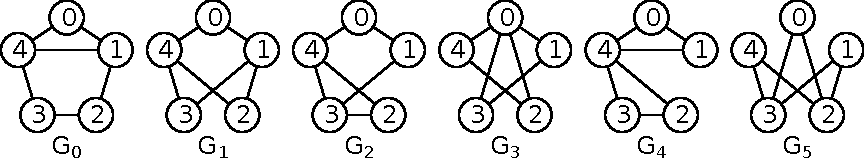
\includegraphics[scale=0.7]{Graphen/Graph_Iso.pdf}
		\end{figure}
	\end{block}
	Tipp: Nach \enquote{markanten} Knoten (Knoten mit hohem Grad) suchen.\\
	Oftmals hierdurch bereits Ausschluss möglich.
\end{frame}

\begin{frame}{Lösung}
	\begin{figure}[H]
		\centering
		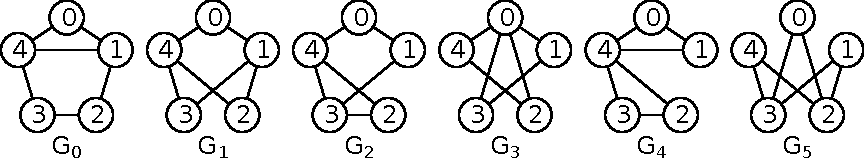
\includegraphics[scale=0.7]{Graphen/Graph_Iso.pdf}
	\end{figure}
	\begin{table}[H]
		\centering
		\begin{tabular}{c|c|c|c|c|c}
			$G_0: $ & 0 & 1 & 2 & 3 & 4 \\
			$G_2: $ & 2 & 3 & 1 & 0 & 4 \\[1em]
			$G_3: $ & 0 & 1 & 2 & 3 & 4 \\
			$G_4: $ & 4 & 0 & 2 & 1 & 3 \\[1em]
			$G_1: $ & 0 & 1 & 2 & 3 & 4 \\
			$G_5: $ & 0 & 2 & 1 & 4 & 3 \\
		\end{tabular}
	\end{table}
\end{frame}

% TODO: Ändern zu Abschnitt über Äquivalenzrelationen in Graphen
%Falls schon Fragen kommen: mit dem Bild einer Nicht-Äquivalenzrelation anfangen und
%so lange Pfeile dazu malen, bis alle Forderungen erfüllt sind:
%• Schlingen an allen Knoten
%• zu jedem Pfeil hin auch der zurück
%• wenn ein Pfad von x nach y existiert, dann auch eine direkte Kante
%Ergebnis: einige Klumpen, äh, Cliquen (die den Äquivalenzklassen entsprechen)

%Pfade, E^*
%• E2 ist wieder Relation auf V: kann man also als Graph malen: Beispiel machen
%• analog für E3, . . .
%• und E^* ist auch wieder eine Relation auf V: kann man also als Graph malen: Beispiel:
%aus Zyklus der Länge 5 wird der sogenannte vollständige Graph K5

%\subsection{Graphen und Relationen}
%\begin{frame}
%	\frametitle{Graphen und Relationen}
%	Wenn $G=(V,E)$ ein (un)gerichteter Graph ist, dann ist $E$ eine binäre Relation. \\ \vspace{2em} \pause
%	Wann ist sie symmetrisch, transitiv, reflexiv? Bzw. was bedeutet das? \\ \vspace{2em} \pause 
%	Was ist $E^i$? Was ist $E^\ast$? Was heißt $E^\ast = V \times V$? 
%\end{frame}

\begin{frame}{Gerichtete Bäume}
	\begin{Definition}
		Ein gerichteter Graph $T$ heißt \textbf{Baum} :{\Gdw} Es gibt eine \textbf{Wurzel} $r \in V$, sodass zu jedem Knoten \emph{genau ein Pfad} von $r$ aus existiert. \\
		\smallskip
		Diese Wurzel ist eindeutig und hat Eingangsgrad $= 0$. \\
		\textbf{Blätter} sind Knoten mit Ausgangsgrad $= 0$. \\
		\textbf{Innere Knoten} sind Knoten mit Ausgangsgrad $> 0$. 
		
	\end{Definition}
\end{frame}

\begin{frame}{Ungerichtete Bäume}
	\begin{Definition}
		Ein ungerichteter Graph $T$ heißt \textbf{Baum} :{\Gdw} Es gibt einen gerichteten Baum, den man zum ungerichteten $T$ umwandeln kann. \\
		\smallskip
		Dessen Wurzel ist \textbf{nicht} eindeutig.
		
	\end{Definition}
\end{frame}

\begin{frame}{Aufgabe: Bäume (WS 2008)}
	\begin{itemize}	
		\item Zeichnen Sie alle möglichen gerichteten Bäume mit genau vier Knoten, von denen keine zwei isomorph sind.
		\item Zeichnen Sie alle möglichen ungerichteten Bäume mit genau fünf Knoten, von denen keine zwei isomorph sind.
	\end{itemize}
\end{frame}

\begin{frame}{Lösung}
	\textit{Zeichnen Sie alle möglichen gerichteten Bäume mit genau vier Knoten, von denen keine zwei isomorph sind.} \pause
	\begin{center}
		\begin{minipage}{0.3\linewidth}
			\vspace*{\fill}
			\centering
			
\includegraphics[scale=0.2]{Graphen/baume1.pdf} 
			\vfill
		\end{minipage}
		\begin{minipage}{0.2\linewidth}
			\vspace*{\fill}
			\centering
			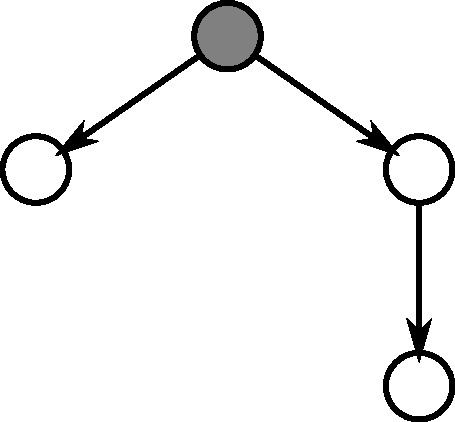
\includegraphics[scale=0.2]{Graphen/baume2.pdf} 
			\vfill
		\end{minipage}
		\begin{minipage}{0.2\linewidth}
			\vspace*{\fill}
			\centering
			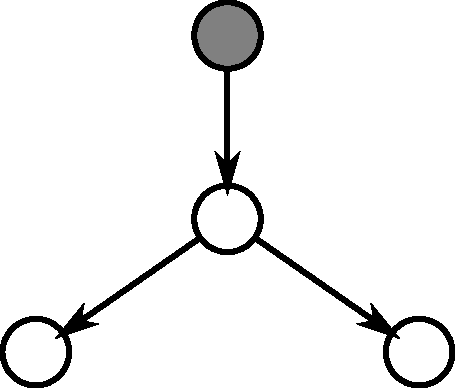
\includegraphics[scale=0.2]{Graphen/baume3.pdf} 
			\vfill
		\end{minipage}
		\begin{minipage}{0.2\linewidth}
			\vspace*{\fill}
			\centering
			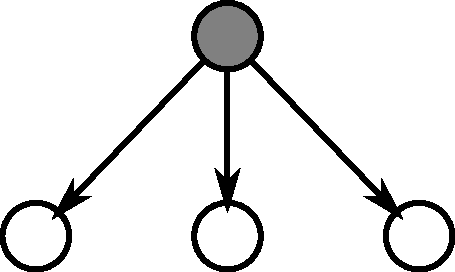
\includegraphics[scale=0.2]{Graphen/baume4.pdf} 
			\vfill
		\end{minipage}
	\end{center} \pause
	\textit{Zeichnen Sie alle möglichen ungerichteten Bäume mit genau fünf Knoten, von denen keine zwei isomorph sind.} \pause
	\begin{center}
		\begin{minipage}{0.2\linewidth}
			\vspace*{\fill}
			\centering
			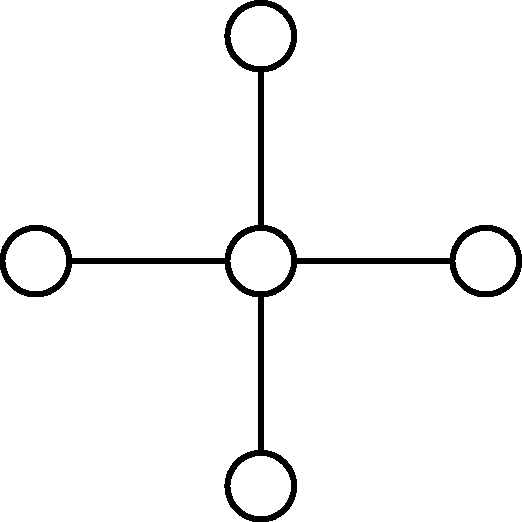
\includegraphics[scale=0.2]{Graphen/baume5.pdf} 
			\vfill
		\end{minipage}
		\begin{minipage}{0.25\linewidth}
			\vspace*{\fill}
			\centering
			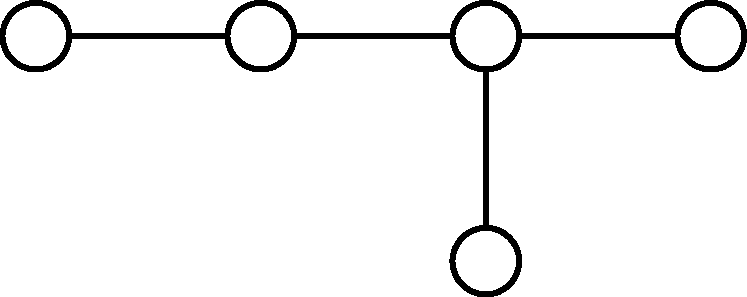
\includegraphics[scale=0.2]{Graphen/baume6.pdf} 
			\vfill
		\end{minipage}
		\begin{minipage}{0.35\linewidth}
			\vspace*{\fill}
			\centering
			
\includegraphics[scale=0.2]{Graphen/baume7.pdf} 
			\vfill
		\end{minipage}
	\end{center}
\end{frame}


\begin{frame}{Aufgabe: Bäume (WS 2010)}
	Sei $T_1 = (V_1 , E_1 )$ ein gerichteter Baum mit Wurzel $r_1$, $T_2 = (V_2 , E_2 )$ ein gerichteter Baum mit Wurzel $r_2$, und es gelte $V_1 \cap V_2 = \{\}$. Sei $r \not\in V_1 \cup V_2$. \\
Zeigen Sie: $$T_1 \circ_r T_2 = (V_1 \cup V_2 \cup {r}, E_1 \cup E_2 \cup \{(r, r_1 ), (r, r_2 )\})$$ ist ein gerichteter Baum mit Wurzel $r$.
\end{frame}

\begin{frame}{Lösung}
	\textit{Zeigen Sie: $$T_1 \circ_r T_2 = (V_1 \cup V_2 \cup {r}, E_1 \cup E_2 \cup \{(r, r_1 ), (r, r_2 )\})$$ ist ein gerichteter Baum mit Wurzel $r$.} \\[2em] \pause
	Zwei Dinge sind zu zeigen:
	\begin{itemize}[<+->]
		\item Zu jedem $v \in V_1 \cup V_2 \cup {r}$ gibt es einen Pfad von $r$ aus
		\item Dieser Pfad ist eindeutig.
	\end{itemize}
\end{frame}

\begin{frame}{Lösung}
	\textit{Wir zeigen zuerst, dass es von $r$ zu jedem Knoten $v \in V_1 \cup V_2 \cup \{r\}$ einen Pfad
gibt.} \\[2em]
	\pause
	\begin{itemize}[<+->]
		\item Es gibt offensichtlich einen Pfad (der Länge 0) von $r$ nach $r$.
		\item Sei $v \in V_1$. Dann gibt es nach Definition einen Pfad von $r_1$ nach $v$ über den Baum $T_1$ und dessen Kanten $E_1$. Da in $T_1 \circ_r T_2$ auch der Pfad $r$ nach $r_1$ liegt, gibt es also einen Pfad von $r$ nach $v$ in $T_1 \circ_r T_2$.
		\item Analog zu $v \in V_2$.
	\end{itemize}
	\visible<5>{Somit gibt es für alle Knoten $v \in V_1 \cup V_2 \cup \{r\}$ einen Pfad von $r$ nach $v$.}
\end{frame}

\begin{frame}{Lösung}
	\textit{Wir zeigen nun noch, dass es für keinen Knoten zwei verschiedenen Pfade von r nach v gibt.} \\[2em]\pause
	Für $v = r$ gibt es offensichtlich keine zwei verschiedenen Pfade. \pause \\ Sei also exemplarisch $v \in V_1$. Da $V_1 \cap V_2 = \{\}$, sind von $r_2$ nur Elemente aus $V_2$ zu erreichen. Somit muss ein Pfad von $r$ nach $v$ über $r_1$ gehen (weil von $r_2$ kein Pfad zurück führt). \pause Da $T_1$ aber ein Baum ist, ist der Pfad von $r_1$ nach $v$ eindeutig. Der Pfad von $r$ nach $r_1$ ebenso. \pause Also ist der Pfad von $r$ nach $v$ auch eindeutig. Analog zu $v \in V_2$.
\end{frame}

% Pufferaufgabe
% Erst einmal weg damit, sowieso keine Zeit und zu schwer fürs Tut
\mycomment{
\begin{frame}{Aufgabe (WS 2009) \stars{4}}
	Eine Zahl $n$ ist genau dann eine Primzahl, wenn sie eine positive ganze Zahl ist und genau zwei Teiler hat, nämlich 1 und n. Insbesondere ist 1 keine Primzahl. \\
	Für $n \in \N^+$ sei der Graph $G_n = (V_n , E_n )$ gegeben durch
	$$V_n =\set{m \in \N^+ \Mid m \text{ teilt } n} \quad \text{und}$$
	$$E_n =\set{(k, m) \in V_n \times V_n \Mid k \text{ teilt } m \text{ und } m/k  \text{ ist eine Primzahl}}.$$
	\begin{itemize}
		\item Zeichnen Sie $G_{12}$ , $G_{16}$ und $G_{30}$.
		\item Zeigen Sie: $$\forall n, m \in \N^+: n \text{ teilt } m \impl G_n \text{ ist Teilgraph von } G_m.$$
	\end{itemize}
\end{frame}

\begin{frame}{Lösung}
	$$V_n =\set{m \in \N^+ \Mid m \text{ teilt } n}, $$
	$$E_n =\set{(k, m) \in V_n \times V_n \Mid k \text{ teilt } m \text{ und } m/k  \text{ ist eine Primzahl}}.$$
	\textit{Zeichnen Sie $G_{12}$ , $G_{16}$ und $G_{30}$.} \\[1,5em]
	
	\visible<2>{
		\begin{center}
			\begin{minipage}{0.2\linewidth}
				\vspace*{\fill}
				\centering
				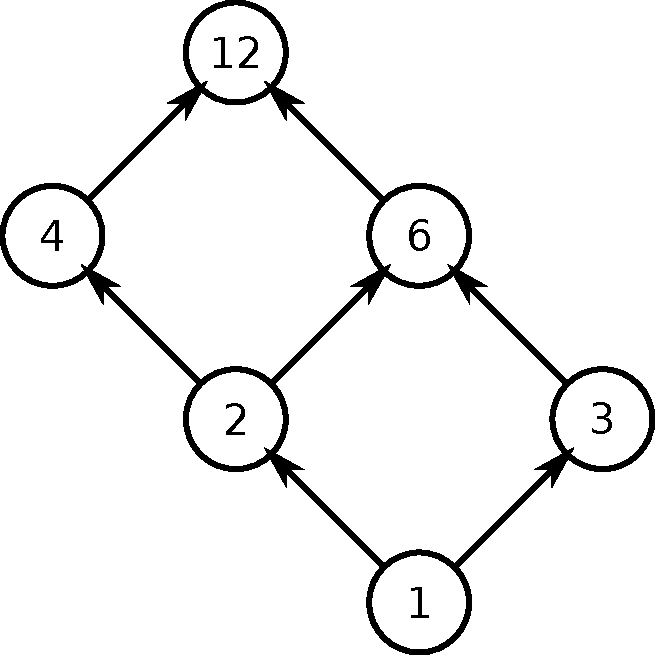
\includegraphics[scale=0.2]{Graphen/Primzahlen1.pdf} 
				\vfill
			\end{minipage}
			\begin{minipage}{0.5\linewidth}
				\vspace*{\fill}
				\centering
				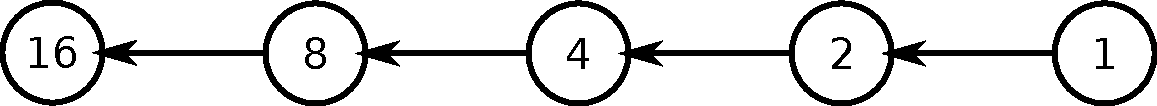
\includegraphics[scale=0.2]{Graphen/Primzahlen2.pdf} 
				\vfill
			\end{minipage}
			\begin{minipage}{0.2\linewidth}
				\vspace*{\fill}
				\centering
				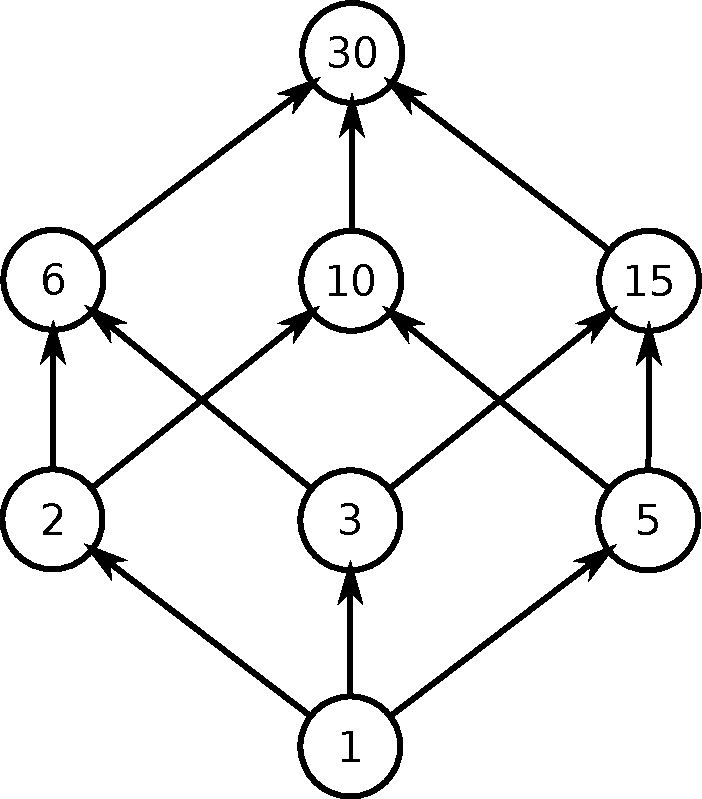
\includegraphics[scale=0.2]{Graphen/Primzahlen3.pdf} 
				\vfill
			\end{minipage}
		\end{center}	
	}
\end{frame}	

\begin{frame}{Lösung}
	\only<1|handout:1>{$G_{12}$}\only<2|handout:2>{$G_{16}$}\only<3|handout:3>{$G_{30}$}
	\vspace*{\fill}
	\centering
	\only<1|handout:1>{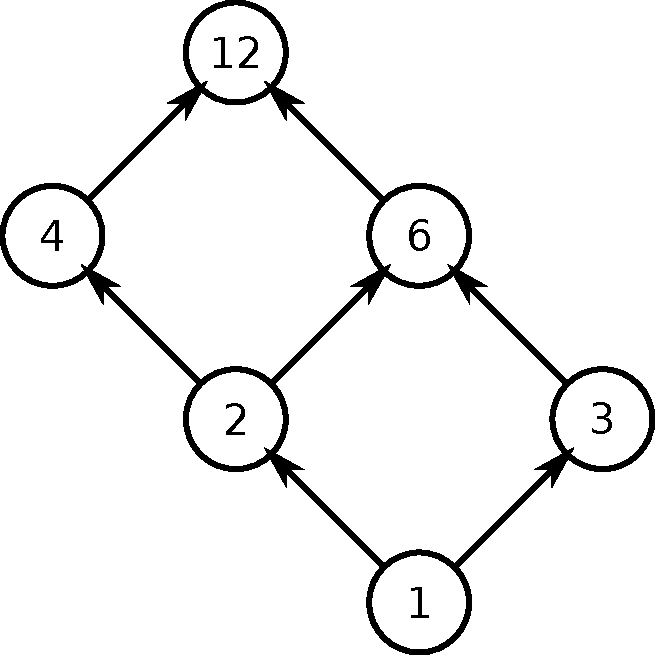
\includegraphics[scale=0.5]{Graphen/Primzahlen1.pdf}}
	\only<2|handout:2>{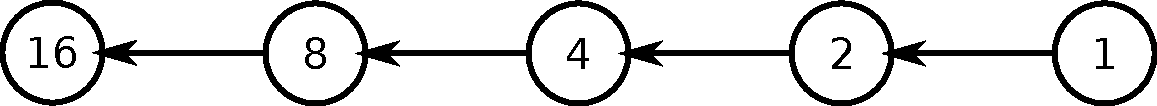
\includegraphics[scale=0.5]{Graphen/Primzahlen2.pdf}}
	\only<3|handout:3>{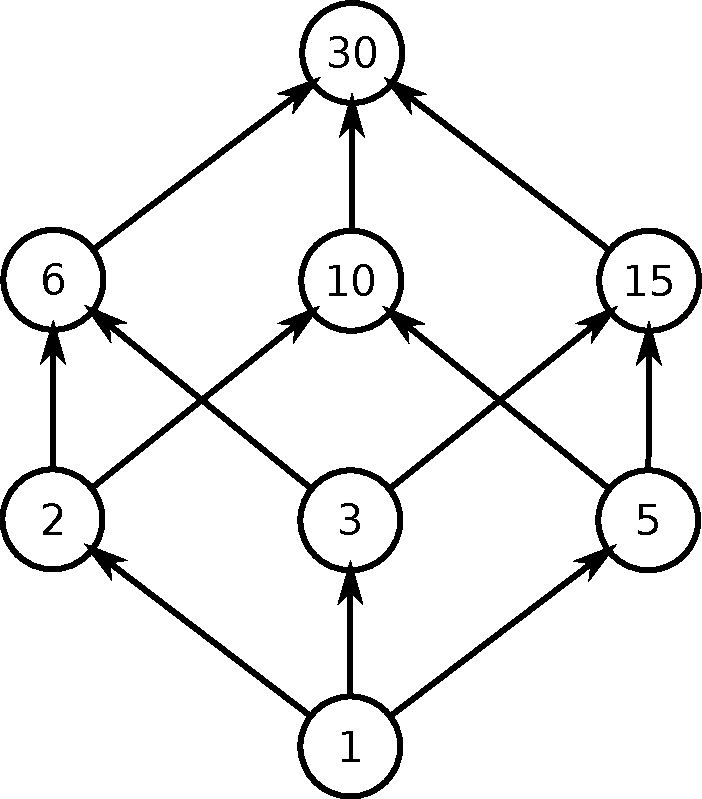
\includegraphics[scale=0.5]{Graphen/Primzahlen3.pdf}}
	\vfill
\end{frame}	

\begin{frame}{Lösung}
	\textit{Zeigen Sie: $$\forall n, m \in \N^+: n \text{ teilt } m \impl G_n \text{ ist Teilgraph von } G_m.$$}\\[2em] \pause
	Gelte also $n$ teilt $m$. Zu zeigen sind zwei Dinge:
	\begin{itemize}
		\item $V_n \subseteq V_m$
		\item $E_n \subseteq E_m \cap V_n \times V_n$
	\end{itemize}
	
\end{frame}

\begin{frame}{Lösung}
	\textit{Zuerst $V_n \subseteq V_m$.} \\[1em] \pause
	Sei $v \in V_n$ beliebig. Nach Definition gilt: $v$ teilt $n$. Da $n$ aber $m$ teilt, muss $v$ auch $m$ teilen, liegt also in $V_m$. Also gilt $$V_n \subseteq V_m$$ \pause
	
	\textit{Jetzt $E_n \subseteq E_m \cap V_n \times V_n$.} \\[1em] \pause
	Sei $p$ eine Kante mit $p = (x,y) \in E_n$. Wir haben gezeigt, dass dann $x,y \in V_m$ gilt. Außerdem gilt nach der Definition von $E_n$: $$x \text{ teilt } y \text{ und } y/x \text{ ist eine Primzahl}$$ Somit ist $p$ auch in $E_m$ und es gilt $$E_n \subseteq E_m$$.
\end{frame}
}